\documentclass[journal,transmag]{IEEEtran}

% Codificación y español
\usepackage[utf8]{inputenc}
\usepackage[T1]{fontenc}
\usepackage[spanish,es-tabla]{babel}

% Matemáticas
\usepackage{amsmath}

% Gráficos
\usepackage{graphicx}

% Tablas
\usepackage{booktabs}
\usepackage{array}
\usepackage{tabularx}
\usepackage{colortbl}

%Código fuente
\usepackage{listings}
\usepackage{xcolor}
\lstset{
  basicstyle=\ttfamily\footnotesize,
  backgroundcolor=\color{gray!10},
  frame=single,
  breaklines=true,
  captionpos=b
}

% ── Hipervínculos ────────────────────────────────────────────
\usepackage{url}

% ── Diagramas TikZ ───────────────────────────────────────────
\usepackage{tikz}
\usetikzlibrary{shapes.geometric, arrows.meta, positioning, calc}

\hyphenation{op-tical net-works semi-conduc-tor}

% ============================================================
%  TÍTULO
% ============================================================
\title{Sistema IoT de Monitoreo Predictivo para Fresadora CNC
mediante Inferencia Edge~AI y Arquitectura Serverless}

% ============================================================
%  AUTORES  (formato transmag: refs compartidas)
% ============================================================
\author{
  \IEEEauthorblockN{
    Valentina L\'opez Maldonado\IEEEauthorrefmark{1},\,
    David Caicedo Sambon\'i\IEEEauthorrefmark{1},\, y\,
    Ktalyna Garc\'ia Benavides\IEEEauthorrefmark{1}%
  }
  \IEEEauthorblockA{%
    \IEEEauthorrefmark{1}%
    \textit{Especializaci\'on en Inteligencia Artificial aplicada a Internet de las Cosas},
    Universidad Aut\'onoma de Occidente, Cali, Colombia.\\
    \{valentina.lnpez,\,david.caicedo\_sam,\,ktalyna.garcia\}@uao.edu.co
  }%

}

% Cabecera de página
\markboth{Especializaci\'on en IA -- Universidad Aut\'onoma de Occidente,~2026}%
{L\'opez \MakeLowercase{\textit{et al.}}: Sistema IoT de Monitoreo Predictivo para Fresadora CNC}

%
%  RESUMEN Y PALABRAS CLAVE
%
\IEEEtitleabstractindextext{%
\begin{abstract}
Este trabajo presenta un sistema de Internet de las Cosas~(IoT) para el monitoreo en tiempo real de una fresadora CNC utilizada en la manufactura de circuitos impresos~(PCBs). El sistema integra un microcontrolador ESP32-C3 con un acel\'erometro MPU-6050 y un sensor de temperatura y humedad DHT22, ejecutando en el borde de la red (\textit{edge}) un modelo de aprendizaje autom\'atico basado en un Perceptr\'on Multicapa~(MLP) entrenado y desplegado con Edge~Impulse, compilado mediante su EON~Compiler sobre TensorFlow~Lite~Micro. El modelo clasifica el estado operativo de la m\'aquina en tres categor\'ias ---reposo, operaci\'on normal y anomal\'ia--- a partir de ocho caracter\'isticas de entrada derivadas de las se\~nales del acel\'erometro. Los datos se transmiten mediante el protocolo~MQTT (MQTTS directo a Azure~IoT~Hub) hacia un \textit{backend} serverless implementado en Azure~Functions~(Python), donde se procesan, almacenan en Azure~Cosmos~DB en modalidad serverless, y generan notificaciones en tiempo real v\'ia la API de Telegram ante la detecci\'on de condiciones an\'omalas. La arquitectura seleccionada prioriza el bajo costo operativo, la escalabilidad y la velocidad de prototipado frente a alternativas convencionales como m\'aquinas virtuales, InfluxDB y servicios de mensajer\'ia de pago. El modelo embebido opera con una arena de tensores de aproximadamente 2\,636~bytes, siendo viable en hardware de bajo costo.
\end{abstract}

\begin{IEEEkeywords}
IoT, Edge~AI, Serverless, Azure~Functions, Cosmos~DB, CNC,
detecci\'on de anomal\'ias, TensorFlow~Lite~Micro, MQTT, PCB.
\end{IEEEkeywords}}

% ============================================================
\begin{document}

\maketitle

\IEEEdisplaynontitleabstractindextext
\IEEEpeerreviewmaketitle

% ============================================================
%  I. INTRODUCCIÓN
% ============================================================
\section{Introducci\'on}

\IEEEPARstart{L}{a} manufactura de circuitos impresos~(PCBs) mediante fresado CNC es un proceso de alta precisi\'on en el que las desviaciones t\'ermicas y las vibraciones an\'omalas ---causadas por desgaste de la herramienta de corte o desalineaci\'on del husillo--- pueden arruinar placas de cobre costosas y romper fresas en cuesti\'on de segundos~\cite{tao2018}. La detecci\'on temprana de estas condiciones es cr\'itica para reducir el desperdicio de material y los tiempos de inactividad no planificados.

Las soluciones de monitoreo industrial convencionales dependen de hardware
propietario costoso o de arquitecturas en la nube basadas en m\'aquinas virtuales permanentemente activas, lo que las hace inaccesibles para talleres de peque\~na escala o contextos acad\'emicos con presupuesto limitado. El paradigma del \textit{Edge~AI} ---la ejecuci\'on de modelos de inferencia directamente en el microcontrolador--- combinado con servicios serverless en la nube representa una v\'ia de soluci\'on de bajo costo y alta escalabilidad~\cite{warden2020}.

El presente trabajo propone e implementa un sistema integral que cubre la cadena completa: adquisici\'on de se\~nales f\'isicas, inferencia en el borde,transmisi\'on ligera de datos, procesamiento serverless, persistencia eficiente y visualizaci\'on en un dashboard~web. La arquitectura est\'a dise\~nada para recibir de forma modular una segunda unidad ESP32-CAM con visi\'on artificial sin requerir cambios en el \textit{backend} ni en el esquema de almacenamiento.


%  II. ARQUITECTURA DEL SISTEMA

\section{Arquitectura del Sistema}

\subsection{Descripci\'on General}

El sistema se organiza en cuatro capas funcionales, tal como se muestra en
la~Fig.~\ref{fig:arquitectura}:

\begin{enumerate}
  \item \textbf{Capa de hardware y Edge~AI:} nodo ESP32-C3 con sensores
        MPU-6050 y DHT22, inferencia TFLite~Micro.
  \item \textbf{Capa de comunicaci\'on:} protocolo MQTT sobre TLS (MQTTS).
  \item \textbf{Capa de c\'omputo serverless:}
        Azure~IoT~Hub $\rightarrow$ Azure~Functions $\rightarrow$ Azure~Cosmos~DB.
  \item \textbf{Capa de presentaci\'on y alertas:} dashboard web est\'atico y
        notificaciones por Telegram.
\end{enumerate}

\begin{figure}[!t]
\centering
\begin{tikzpicture}[
  node distance = 5mm and 6mm,
  box/.style    = {draw, rounded corners=2pt, minimum width=3.0cm,
                   minimum height=0.6cm, align=center, font=\footnotesize},
  arrow/.style  = {-Stealth, thick}
]
  \node[box, fill=blue!15]   (esp) {ESP32-C3\\MPU-6050 + DHT22\\TFLite MLP};
  \node[box, fill=orange!20, below=of esp] (hub) {Azure IoT Hub};
  \node[box, fill=green!20,  below=of hub] (fn)  {Azure Functions (Python)};
  \node[box, fill=purple!20, below=of fn]  (db)  {Azure Cosmos DB Serverless};
  \node[box, fill=cyan!15,   below=of db]  (fe)  {Dashboard Web};
  \node[box, fill=yellow!25, right=16mm of fn] (tg) {Telegram Bot API};

  \draw[arrow] (esp) -- node[right,font=\tiny]{MQTTS} (hub);
  \draw[arrow] (hub) -- node[right,font=\tiny]{Event Hub trigger} (fn);
  \draw[arrow] (fn)  -- node[right,font=\tiny]{Cosmos SDK} (db);
  \draw[arrow] (db)  -- node[right,font=\tiny]{REST} (fe);
  \draw[arrow] (fn)  -- node[above,font=\tiny]{Alerta} (tg);
\end{tikzpicture}
\caption{Arquitectura completa del sistema de monitoreo CNC.}
\label{fig:arquitectura}
\end{figure}

\subsection{Capa de Hardware}

El nodo principal est\'a basado en un ESP32-C3~DevKit, seleccionado por su soporte nativo de WiFi~802.11~b/g/n, perif\'ericos I2C/GPIO y bajo costo ($\approx$\$4~USD). La Fig.~\ref{fig:circuito} muestra el diagrama de conexiones del circuito y la Tabla~\ref{tab:conexiones} resume las conexiones f\'isicas, conforme a la configuraci\'on del firmware (\texttt{config.h}).

\begin{figure}[!t]
\centering
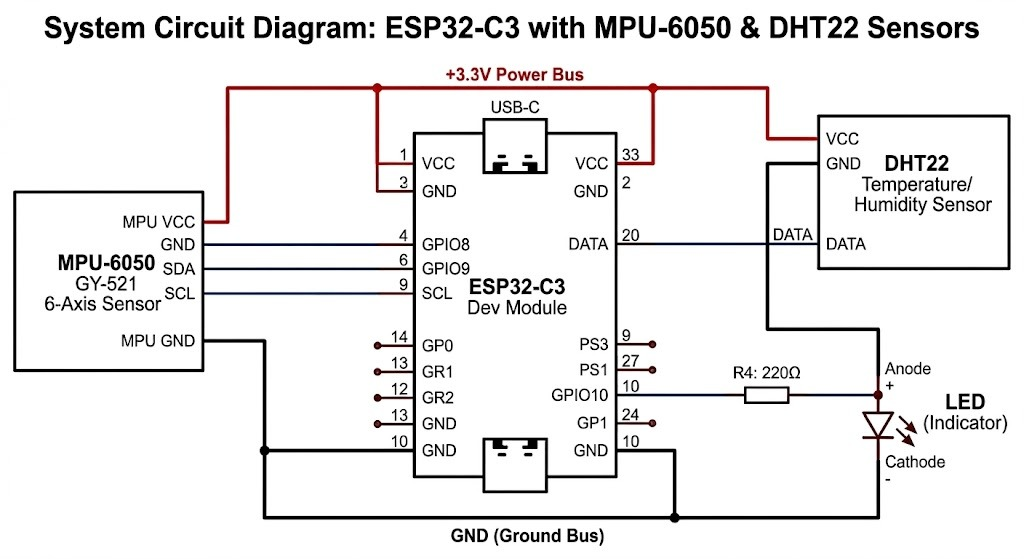
\includegraphics[width=\columnwidth]{img/diagrama_circuito.jpeg}
\caption{Diagrama de conexiones del nodo principal: ESP32-C3 con MPU-6050
(I2C), DHT22 y LED indicador.}
\label{fig:circuito}
\end{figure}

\begin{table}[!t]
\caption{Conexiones f\'isicas del nodo principal}
\label{tab:conexiones}
\centering
\renewcommand{\arraystretch}{1.2}
\begin{tabular}{lll}
\toprule
\textbf{Componente} & \textbf{Protocolo} & \textbf{Pines ESP32-C3} \\
\midrule
MPU-6050 & I2C (dir.\ 0x68)  & SDA: GPIO~8 / SCL: GPIO~9 \\
DHT22    & 1-Wire             & GPIO~0 (pull-up 10\,k$\Omega$) \\
LED estado & Salida digital   & GPIO~10 \\
\bottomrule
\end{tabular}
\end{table}

El acel\'erometro se configura en el rango $\pm2\,g$, con una sensibilidad de 16\,384~LSB/g. Las muestras de aceleraci\'on se acumulan y se transforman en el vector de caracter\'isticas que alimenta al modelo.

\subsection{Modelo de Aprendizaje Autom\'atico}

Se emple\'o un Perceptr\'on Multicapa~(MLP) entrenado y exportado desde Edge~Impulse, compilado mediante el EON~Compiler al formato de TensorFlow~Lite~Micro. Las ocho caracter\'isticas de entrada se detallan en la Tabla~\ref{tab:features}.

\begin{table}[!t]
\caption{Caracter\'isticas de entrada del modelo MLP}
\label{tab:features}
\centering
\renewcommand{\arraystretch}{1.2}
\begin{tabular}{cll}
\toprule
\textbf{\#} & \textbf{S\'imbolo} & \textbf{Descripci\'on} \\
\midrule
0 & $\bar{a}_x$      & Media de aceleraci\'on en eje~X \\
1 & $\sigma^2_{a_x}$ & Varianza de aceleraci\'on en eje~X \\
2 & $\bar{a}_y$      & Media de aceleraci\'on en eje~Y \\
3 & $\sigma^2_{a_y}$ & Varianza de aceleraci\'on en eje~Y \\
4 & $\bar{a}_z$      & Media de aceleraci\'on en eje~Z \\
5 & $\sigma^2_{a_z}$ & Varianza de aceleraci\'on en eje~Z \\
6 & $T$              & Temperatura ambiente (°C) \\
7 & $H$              & Humedad relativa (\%) \\
\bottomrule
\end{tabular}
\end{table}

El modelo clasifica en tres clases: \textbf{reposo}, \textbf{operaci\'on normal} y \textbf{anomal\'ia}, y se ejecuta sobre una arena de tensores de aproximadamente 2\,636~bytes, viable en el ESP32-C3.

%  III. IMPLEMENTACIÓN

\section{Implementaci\'on}

\subsection{Firmware (ESP32-C3)}

El firmware se desarroll\'o en C++ con el \textit{framework} Arduino e incluye
las bibliotecas: el \textbf{SDK exportado de Edge~Impulse}
(\texttt{CNC\_Monitor\_Project\_inferencing}), \texttt{DHT}, \texttt{Wire},
\texttt{WiFiClientSecure}, \texttt{PubSubClient}, \texttt{ArduinoJson} y
\texttt{mbedTLS}. La inferencia se realiza mediante la funci\'on
\texttt{run\_classifier()} provista por el SDK, que integra el preprocesamiento
DSP y la red neuronal. El ciclo de operaci\'on es:

\begin{enumerate}
  \item Al arranque: inicializaci\'on de WiFi, sincronizaci\'on NTP,
        conexi\'on MQTTS a Azure~IoT~Hub y carga del modelo Edge~Impulse.
  \item En el bucle principal: lectura del acel\'erometro y
        acumulaci\'on en el b\'ufer de entrada del modelo.
  \item Al completar la ventana: extracci\'on de caracter\'isticas
        $\rightarrow$ inferencia $\rightarrow$ publicaci\'on MQTT.
  \item Periodicamente: lectura de temperatura y humedad del DHT22 (cada 2~s)
        y publicaci\'on de telemetr\'ia al cloud (cada 5~s).
\end{enumerate}

La conexi\'on se establece directamente contra Azure~IoT~Hub mediante MQTTS
(puerto~8883), autenticada con un token~SAS generado en el dispositivo con
HMAC-SHA256 (mbedTLS). El \textit{payload} MQTT sigue el contrato JSON del
Listado~\ref{lst:json}.

\begin{lstlisting}[caption={Contrato JSON del payload MQTT.},label={lst:json}]
{
  "device_id": "cnc_fresadora_01",
  "timestamp": 1716076800,
  "sensors": {
    "temperature": 24.5,
    "humidity": 45.2,
    "vibration_status": "normal"
  },
  "predictions": {
    "vibration_anomaly_score": 0.02,
    "visual_anomaly_score": null
  }
}
\end{lstlisting}

El campo \texttt{visual\_anomaly\_score} queda reservado en \texttt{null} para la futura integraci\'on de la ESP32-CAM sin romper el esquema existente.

\subsection{Backend Serverless (Azure Functions)}

Se implementaron cinco funciones en Python:

\begin{itemize}
  \item \textbf{\texttt{telemetry\_processor}}: trigger de Event~Hub.
        Parsea el payload, eval\'ua umbrales y persiste el documento en
        Cosmos~DB mediante el SDK oficial de Azure~Cosmos.
  \item \textbf{\texttt{get\_datos}} (GET \texttt{/api/datos}): retorna los
        \'ultimos $N$ registros con filtrado por dispositivo.
  \item \textbf{\texttt{descargar\_csv}} (GET \texttt{/api/datos/csv}):
        exporta el historial en formato CSV.
  \item \textbf{\texttt{control\_actuador}} (POST \texttt{/api/actuador}):
        env\'ia comandos ON/OFF/RESET al ESP32 mediante tres m\'etodos en
        cascada: Direct~Method, C2D~SDK y REST~C2D con token~SAS.
  \item \textbf{\texttt{ingestar\_camara}} (POST \texttt{/api/camara}):
        \textit{endpoint} ya preparado para recibir las clasificaciones de la
        futura ESP32-CAM, evidenciando la modularidad del dise\~no.
\end{itemize}

\subsection{Sistema de Alertas}

Cuando el \textit{score} de anomal\'ia supera el umbral configurable
(por defecto 0.80) o los valores de temperatura y humedad exceden sus rangos
normales (15--45\,°C y 20--80\,\%, respectivamente), la funci\'on
\texttt{telemetry\_processor} realiza un HTTP~POST a la API de Telegram,
entregando una notificaci\'on instant\'anea con los valores del evento.


%  IV. JUSTIFICACIÓN DE LA ARQUITECTURA

\section{Justificaci\'on de la Arquitectura}

La selecci\'on de cada componente responde a tres pilares:
\textbf{bajo costo operativo, rapidez de prototipado y escalabilidad futura}.

\subsection{C\'omputo Serverless vs.\ M\'aquinas Virtuales}

Se adopt\'o \textbf{Azure~Functions en plan de consumo} en lugar de m\'aquinas virtuales o contenedores Docker permanentes. Una~VM activa 24/7 consume cr\'editos de forma constante, independientemente de si la CNC est\'a operando o no. El modelo serverless factura \'unicamente por ejecuci\'on real: si el equipo est\'a apagado, el costo es \$0. Azure incluye adem\'as el primer mill\'on de ejecuciones mensuales de forma gratuita~\cite{azure_pricing}, cubriendo ampliamente el volumen esperado. Las credenciales se gestionan mediante variables de entorno encriptadas (\textit{App Settings}), evitando la exposici\'on de secretos en el c\'odigo fuente.

\subsection{Protocolo MQTT vs.\ HTTP}

HTTP impone una sobrecarga significativa de cabeceras (varios cientos de bytes por petici\'on), mayor consumo de RAM y tiempo de procesamiento en el microcontrolador~\cite{mqtt_spec}. MQTT es un protocolo binario con cabecera m\'inima de 2~bytes, dise\~nado para dispositivos con recursos limitados. El patr\'on \textit{publicador/suscriptor} permite que el firmware publique el
dato y se desentienda de su entrega; el \textit{broker} (Azure~IoT~Hub)
distribuye la informaci\'on hacia m\'ultiples consumidores de forma eficiente.

\subsection{Cosmos~DB Serverless vs.\ InfluxDB vs.\ PostgreSQL}

\begin{itemize}
  \item \textbf{InfluxDB} es \'optimo para series de tiempo, pero requiere un servidor dedicado con funcionamiento continuo, elevando el costo.
  \item \textbf{PostgreSQL} exige gesti\'on de esquemas y \textit{pools} de conexiones desde funciones serverless, a\~nadiendo complejidad operativa.
  \item \textbf{Cosmos~DB Serverless} factura por Unidades de
        Petici\'on~(RUs) consumidas, sin cargo base. Azure~Functions ofrece
        adem\'as \textit{Output~Bindings} nativos para Cosmos~DB que reducen el
        c\'odigo de persistencia~\cite{cosmos_binding}. El esquema flexible de
        JSON facilita incorporar \texttt{visual\_anomaly\_score} en el futuro
        sin migraciones.
\end{itemize}

\subsection{Telegram vs.\ Correo Electr\'onico / SMS}

La API de Telegram es completamente gratuita, as\'incrona y de baja
latencia~\cite{telegram_api}. El env\'io de una notificaci\'on se reduce a una petici\'on HTTP~POST con la biblioteca est\'andar \texttt{requests}, sin dependencias adicionales, a diferencia de SendGrid o~Twilio, que requieren credenciales de pago o configuraciones DNS.

\subsection{Matriz de Decisiones}

La Tabla~\ref{tab:matriz} sintetiza las decisiones arquitect\'onicas.

\begin{table}[!t]
\caption{Matriz de decisiones arquitect\'onicas}
\label{tab:matriz}
\centering
\renewcommand{\arraystretch}{1.2}
\begin{tabularx}{\columnwidth}{p{1.4cm} p{1.7cm} X}
\toprule
\textbf{Capa} & \textbf{Tecnolog\'ia} & \textbf{Raz\'on principal} \\
\midrule
Firmware      & C++ + Edge Impulse SDK        & Bajo consumo de RAM, inferencia TFLite integrada \\
C\'omputo     & Azure Functions Serverless     & Costo \$0 en inactividad \\
Persistencia  & Cosmos DB Serverless           & Esquema flexible, sin cargo base \\
Comunicaci\'on & MQTT (MQTTS)                  & Cabecera m\'inima, menor consumo energ\'etico \\
Alertas       & Telegram Bot API               & Gratuito, latencia baja \\
\bottomrule
\end{tabularx}
\end{table}


%  V. RESULTADOS

\section{Resultados}

\subsection{M\'etricas del Modelo de Clasificaci\'on}

El modelo MLP fue entrenado sobre un \textit{dataset} balanceado de 468~muestras
(156 por clase) recolectadas directamente de la fresadora CNC en las tres
condiciones operativas definidas. La evaluaci\'on se realiz\'o mediante
validaci\'on \textit{hold-out} estratificada (80\,\% entrenamiento, 20\,\%
prueba; 94~muestras de prueba), con normalizaci\'on estándar de las
caracter\'isticas. La Tabla~\ref{tab:metricas} muestra las m\'etricas de
evaluaci\'on por clase.

\begin{table}[!t]
\caption{M\'etricas de evaluaci\'on del clasificador MLP}
\label{tab:metricas}
\centering
\renewcommand{\arraystretch}{1.2}
\begin{tabular}{lccc}
\toprule
\textbf{Clase} & \textbf{Precisi\'on} & \textbf{Recall} & \textbf{F1-Score} \\
\midrule
Reposo           & 0.912 & 1.000 & 0.954 \\
Operaci\'on normal & 1.000 & 0.903 & 0.949 \\
Anomal\'ia        & 1.000 & 1.000 & 1.000 \\
\midrule
\textbf{Promedio} & \textbf{0.971} & \textbf{0.968} & \textbf{0.968} \\
\bottomrule
\end{tabular}
\end{table}

\textbf{Exactitud global (\textit{Accuracy}):} 96.81\,\%.

La Tabla~\ref{tab:confusion} presenta la matriz de confusi\'on sobre el
conjunto de prueba. La diagonal (resaltada) corresponde a las predicciones
correctas; los \'unicos errores fueron tres muestras de operaci\'on normal
clasificadas como reposo, mientras que la clase \textbf{anomal\'ia} ---la m\'as
cr\'itica para el caso de uso--- se detect\'o sin errores (32/32).

\begin{table}[!t]
\caption{Matriz de confusi\'on del clasificador MLP (conjunto de prueba, 94~muestras)}
\label{tab:confusion}
\centering
\renewcommand{\arraystretch}{1.3}
\setlength{\tabcolsep}{5pt}
\begin{tabular}{l|ccc}
\toprule
\textbf{Real\,$\downarrow$ / Pred.\,$\rightarrow$} & \textbf{Reposo} & \textbf{Normal} & \textbf{Anomal\'ia} \\
\midrule
Reposo            & \cellcolor{green!25}31 & 0  & 0 \\
Operaci\'on normal & 3  & \cellcolor{green!25}28 & 0 \\
Anomal\'ia        & 0  & 0  & \cellcolor{green!25}32 \\
\bottomrule
\end{tabular}
\end{table}

La Tabla~\ref{tab:modelo} resume los par\'ametros t\'ecnicos del modelo.

\begin{table}[!t]
\caption{Par\'ametros t\'ecnicos del modelo embebido}
\label{tab:modelo}
\centering
\renewcommand{\arraystretch}{1.2}
\begin{tabular}{ll}
\toprule
\textbf{Par\'ametro} & \textbf{Valor} \\
\midrule
Arquitectura           & MLP (capas densas, ReLU + Softmax) \\
Entradas               & 8 caracter\'isticas \\
Clases de salida       & 3 (reposo, normal, anomal\'ia) \\
Tama\~no del modelo    & [COMPLETAR] bytes (FlatBuffer TFLite) \\
Arena de tensores      & 2\,636 bytes (\textit{tensor arena} TFLite) \\
Umbral anomal\'ia LED  & 0.70 \\
Umbral alerta cloud    & 0.80 \\
\bottomrule
\end{tabular}
\end{table}

\subsection{Estimaci\'on de Costo Operativo}

La Tabla~\ref{tab:costo} presenta el costo mensual estimado para una CNC
con $\approx$500~registros/d\'ia.

\begin{table}[!t]
\caption{Costo operativo mensual estimado}
\label{tab:costo}
\centering
\renewcommand{\arraystretch}{1.2}
\begin{tabular}{lc}
\toprule
\textbf{Servicio} & \textbf{USD/mes} \\
\midrule
Azure Functions (primer mill\'on de ejec.)  & \$0.00 \\
Azure Cosmos DB Serverless                   & $<$\$0.10 \\
Azure IoT Hub (Free Tier: 8\,000~msgs/d\'ia) & \$0.00 \\
Azure Static Website (Storage)              & $<$\$0.01 \\
Telegram Bot API                             & \$0.00 \\
\midrule
\textbf{Total}                               & $<$\textbf{\$0.11} \\
\bottomrule
\end{tabular}
\end{table}


%  VI. CONCLUSIONES

\section{Conclusiones}

Se dise\~n\'o e implement\'o un sistema IoT completo para el monitoreo predictivo de una fresadora CNC, demostrando la viabilidad de combinar inferencia Edge~AI en microcontroladores de bajo costo con una arquitectura serverless en la nube. Los aportes principales son:

\begin{enumerate}
  \item El modelo MLP embebido (arena de $\approx$2\,636~bytes) permite la clasificaci\'on en tiempo real en el ESP32-C3, reduciendo la latencia y el ancho de banda frente a inferencia en la nube.
  \item La arquitectura serverless elimina el costo base de infraestructura ($<$\$0.11~USD/mes para una CNC individual).
  \item Las alertas v\'ia Telegram ofrecen notificaciones en tiempo real sin costo adicional, con implementaci\'on en pocas l\'ineas de c\'odigo.
  \item La arquitectura queda preparada para integrar una capa de visi\'on artificial (ESP32-CAM) de forma modular, sin redise\~nar el
        \textit{backend} ni el esquema de almacenamiento, como evidencia el \textit{endpoint} \texttt{/api/camara} ya disponible.
\end{enumerate}

Como trabajo futuro se contempla la integraci\'on de la ESP32-CAM, el
entrenamiento del modelo con un \textit{dataset} de mayor tama\~no y la implementaci\'on de actualizaciones OTA del firmware.


%  REFERENCIAS

\begin{thebibliography}{9}

\bibitem{tao2018}
F.~Tao, Q.~Qi, A.~Liu, y A.~Kusiak,
``Data-driven smart manufacturing,''
\textit{J. Manuf. Syst.}, vol.~48, pp.~157--169, jul. 2018.

\bibitem{warden2020}
P.~Warden y D.~Situnayake,
\textit{TinyML: Machine Learning with TensorFlow Lite on Arduino and
Ultra-Low-Power Microcontrollers}.
O'Reilly Media, 2020.

\bibitem{azure_pricing}
Microsoft Azure, ``Azure Functions pricing,''
[En l\'inea]. Disponible en:
\url{https://azure.microsoft.com/pricing/details/functions/}.
[Accedido: mayo 2026].

\bibitem{mqtt_spec}
A.~Stanford-Clark y H.~L.~Truong,
``MQTT For Sensor Networks (MQTT-SN) Protocol Specification, v1.2,''
MQTT.org, nov. 2013.

\bibitem{cosmos_binding}
Microsoft Azure,
``Azure Cosmos DB output binding for Azure Functions,''
\textit{Azure Functions documentation}, 2024.

\bibitem{telegram_api}
Telegram, ``Telegram Bot API,''
[En l\'inea]. Disponible en: \url{https://core.telegram.org/bots/api}.
[Accedido: mayo 2026].

\bibitem{lecun2015}
Y.~LeCun, Y.~Bengio, y G.~Hinton,
``Deep learning,''
\textit{Nature}, vol.~521, pp.~436--444, 2015.

\end{thebibliography}

\end{document}
